\section{導入}

\begin{frame}{Dockerとは何か?}
    アプリケーション実行環境を構築,共有,起動するための\\ソフトウェアプラットフォーム.

    \begin{figure}
        \centering
        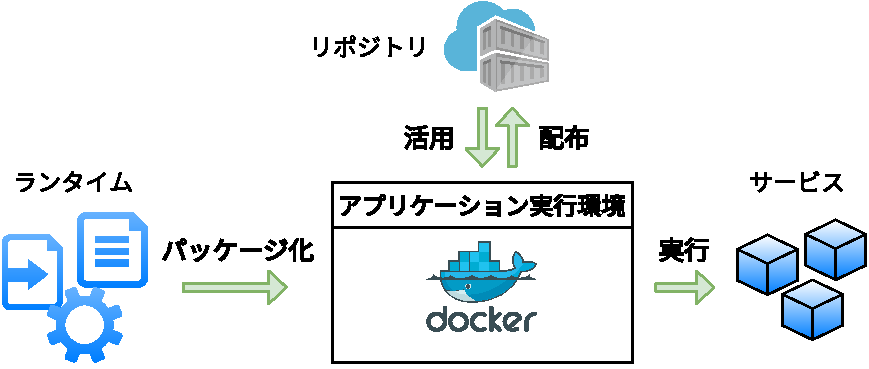
\includegraphics[width=\linewidth]{img/docker.pdf}
    \end{figure}
\end{frame}


\begin{frame}{Dockerfileとは何か?}
    Dockerにおいて,
    \begin{description}
        \item[イメージ] アプリケーション実行環境のスナップショット
        \item[コンテナ] イメージから生成するアプリケーション実行環境
    \end{description}

    Dockerfileは,イメージ構築を自動化する一連の命令列が\\記載されたテキストファイル.

    \begin{columns}[totalwidth=\mytotalwidth]
        \begin{column}[T]{0.05\mycolumnwidth}
        \end{column}
        \begin{column}[T]{0.25\mycolumnwidth}
            \begin{figure}
                \centering
                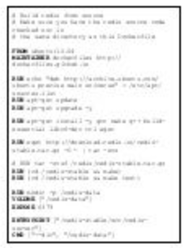
\includegraphics[height=60pt]{img/_dockerfile.png}
                \caption{Dockerfile}
            \end{figure}
        \end{column}
        \begin{column}[T]{0.1\mycolumnwidth}
            \vskip2.0zh
            \centerline{build}
            \centerline{$\longrightarrow$}
        \end{column}
        \begin{column}[T]{0.3\mycolumnwidth}
            \begin{figure}
                \centering
                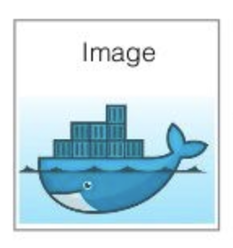
\includegraphics[height=60pt]{img/_image.png}
                \caption{イメージ}
            \end{figure}
        \end{column}
        \begin{column}[T]{0.1\mycolumnwidth}
            \vskip1.0zh
            \centerline{run}
            \centerline{$\longrightarrow$}
            \centerline{\footnotesize (commit)}
            \centerline{$\dashleftarrow$}
        \end{column}
        \begin{column}[T]{0.3\mycolumnwidth}
            \begin{figure}
                \centering
                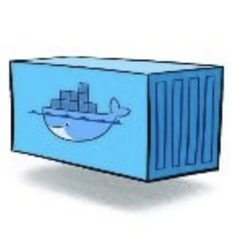
\includegraphics[height=60pt]{img/_container.png}
                \caption{コンテナ}
            \end{figure}
        \end{column}
    \end{columns}
\end{frame}